\documentclass{llncs}

\usepackage{polyglossia}
\setmainlanguage{english}

% \usepackage{natbib}

%\usepackage{fontspec}
%\setmainfont{TeXGyreTermes}

\usepackage{url}

\title{Xodx}
\subtitle{a prove of concept and usability/practicability for the Distributed Semantic Social Network (DSSN)}
\author{}
\institute{\email{\{lastname\}@informatik.uni-leipzig.de}}

\begin{document}
\maketitle

\begin{abstract}
The Distributed Semantic Social Network is a new architecture for online social networks which has many benefits in terms of privacy, data security and data ownership.
The aim of this article is to examine if and how it is possible to setup a node of such a network on low cost and low powered hardware.
This report especially concentrates on the DSSN node implementation Xodx, its architecture and development.
\end{abstract}

\section{Introduction}
Einführung und Motivation aus meiner Masterarbeit

The aim of this paper is to prove that the concept of a DSSN as described in \cite{tramp-s-2012--a} is practically usable to run a social network.
For this purpose this paper introduces Xodx the implementation of a node for the DSSN, which provides the functionality needed for social communication in the Semantic Web.
- Setup testbed of multiple nodes to prove the interoperability


\section{The DSSN}
The Distributed Semantic Social Network (DSSN) is the idea of an architecture of an online social network, which consists of Linked Data RDF-Resources\footnote{See also Resource Description Framework (RDF) \cite{lassila-o-1999--a} and Linked Data \cite{bernerslee-t-2009--}} (from now on just called \emph{resources}), representing persons, which are placed on different nodes distributed across the internet.
Thus each node holds a part of the network information and refers to other nodes.

As proposed in “An Architecture of a Distributed Semantic Social Network” \cite{tramp-s-2012--a} the DSSN is structured into four layers, the data, protocol, service and application layers.
The data layer contains the resources which can represent persons, applications, data- or media-artifacts and Atom-Feeds which are used to represent and publish temporarily ordered activities.
The protocol layer contains the WebID protocol for identification, Semantic Pingback \cite{tramp-s-2010--b} for proactive notifications to resources (e.g. befriending) and PubSubHubbub (PuSH) for resources to be subscribed to Atom-Feeds.
The service layer combines applications which have access for manipulation to the user's data. Until now the ping service, for receiving pings, the PuSH service, for publishing and subscribing to feeds, search and index services are defined.
Finally the application layer allows all different kinds of applications which the user gives access to, to access his data and act in his name.

A node in the DSSN has to understand (beside HTTP) the mentioned protocols (Semantic Pingback and PuSH).
It can provide data (resources and/or feeds) about persons or artifacts in the data layer and/or provide services and applications on the service and application layers either only to the users of this node or also to other users of the DSSN.

\section{Xodx -- a prove of concept and usability/practicability for the Distributed Semantic Social Network}
Because the DSSN should be optimally, from a privacy, data security and data ownership point of view, completely distributed across multiple nodes on the Internet the best would be to have one node per user where the user can control which data and services she wants to provide to others and which services he wants to use on other nodes.
The acceptance to run a personal node can be increased by minimizing the hardware requirements for the software and thus minimizing the costs for the users.

To get closer to this goal the aim of this practical is to examine the basics of a DSSN setup on cheep and low powered hardware and to develop open source software which other users can take to setup there own nodes.

The practical is structured in two groups, one is implementing a DSSN node using Node.js and the other group extended the Xodx project\footnote{Xodx: \url{http://xodx.dssn.org}}, which is based on PHP.

\subsection{Requirements}

\subsection{Architecture}
Xodx is an implementation of the basic functionality of a DSSN node.
On the data layer it can be used for publishing resources and Activity-Feeds.
On the protocol and service layers it can receive Semantic Pingback-Pings and publish and subscribe with PubSubHubbub (PuSH) to Atom-Feeds.
Furthermore on the application layer it has a simple profile manager which can be used to create new person resources and add new friendships to it.
The architecture and intercommunication with other DSSN nodes and services is depicted in Fig. \ref{Xodx_arch}.

Xodx is constructed as a web application according to the Model-View-Controller (MVC) software design pattern which is supported by the Semantic Application Framework Saft\footnote{Semantic Application Framework Saft: \url{https://github.com/white-gecko/Saft}}.
PHP is used as programming language because Xodx makes highly use of the Erfurt Framework\footnote{Erfurt Framework: \url{http://erfurt-framework.org/}} and lib-dssn-php\footnote{lib-dssn-php: \url{https://github.com/AKSW/lib-dssn-php/}}.
A class diagram of Xodx together with Saft can be seen in the appendix.

\begin{figure}
    \begin{center}
        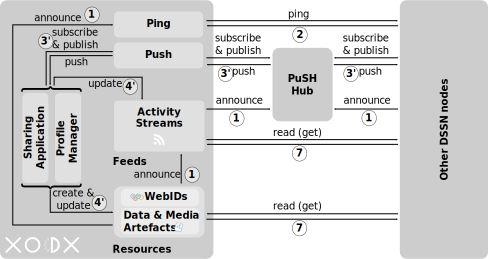
\includegraphics[width=.687\textwidth]{graphics/Xodx-in-DSSN-Architecture}
    \end{center}
\caption{The architecture of Xodx and its integration with other services and nodes}
\label{Xodx_arch}
\end{figure}


\subsection{Results}

\todo{funktionsumfang und vergleich mit Requirements section}

\section{Evaluation of Simulation of semantic driven distributed social networks}

- zweiter Hauptteil hauptteil des papers
- aufbau von test copora (generierung und gathering)
- vokabular für simulation
- simulation (xodx)
- results

\subsection{Test Hardware and Software Environment}
The test hardware which was used for this practical is a Olimex A13-OLinuXino-WIFI board with an ARMv7 Cortex A8 processor at 1GHz (Allwinner A13 System on a chip), 512 MB RAM and 2–8 GB SD-Card-Storage.

The used operating system is a Debian GNU/Linux (arm hard float port, armhf) which was customized to boot and run on the board.
The kernel is a Linux 3.0.42 compiled from the sources provided by the Linux-Sunxi project\footnote{Linux-Sunxi project wiki: \url{http://linux-sunxi.org}, Kernel Sources: \url{https://github.com/linux-sunxi/linux-sunxi}}.

To get a web server environment the very light and resource efficient nginx was used to run PHP applications with the fast-cgi extension.
As database the Open\-Link Vir\-tu\-oso Open-Source Edition\footnote{Open\-Link Vir\-tu\-oso Open-Source: \url{http://ods.openlinksw.com/dataspace/doc/dav/wiki/Main/Main.VOSIndex}} was chosen because it is the best supported back-end for the Erfurt Framework.


\bibliographystyle{splncs03}
\bibliography{library}

\end{document}
